% ══════════════════════════════════════════════════════════════════════════════
% CHAPTER 4 — PROPOSED FRAMEWORK: CHATSERVE
% ══════════════════════════════════════════════════════════════════════════════
\chapter{Proposed Framework -- ChatServe}

\section{System Overview}

ChatServe provides multiple tenants with access to a software as a service (SaaS)-based product that has been created using the Meta WhatsApp Cloud API. It allows small business owners to set up and run a fully automated ordering and booking system via WhatsApp without any technical expertise. The entire platform runs using three components working together seamlessly and collectively provide users with an easy-to-use experience. 

First, there is a new business registration bot for owners to onboard their businesses with ease via WhatsApp, which guides them through the onboarding process; and second, there will be a bot created for each business to assist with customer orders and bookings from the business's WhatsApp business account; and finally, the platform has created web dashboards, one for administrators to manage all platforms' activity and a second for business owners to manage their own operations, and receive reporting on how their businesses are performing and how well they are connecting with customers. This method of using third parties for an ordering and booking system will make it easier for customers to place orders or book services from a business as well as make it easier to manage the day-to-day operations of running the business.

The primary design philosophy behind ChatServe is to ensure that business owners do not have to leave the WhatsApp platform when registering. ChatServe is designed to automatically handle all technical aspects of the registration process once all required authorisations have been granted. As part of this process, the business owner will communicate with the bot, authorise the connection request, then start receiving orders and bookings via WhatsApp.


\section{System Architecture}

ChatServe is a tiered web application which has separate layers for each concern. We have two React SPAs in the Presentation Layer. The API Gateway Layer is an Express.js server which does routing, authentication, and rate limiting. Below that we have Business Logic Layer which includes service modules for each main function. For the Data Layer we use MongoDB (primary data store) and Cloudinary (for media). Also we interface with external services which include Meta WhatsApp Cloud API and Meta Graph API we use webhooks for the former and make outbound HTTPS calls for the latter.

\begin{figure}[H]
\centering
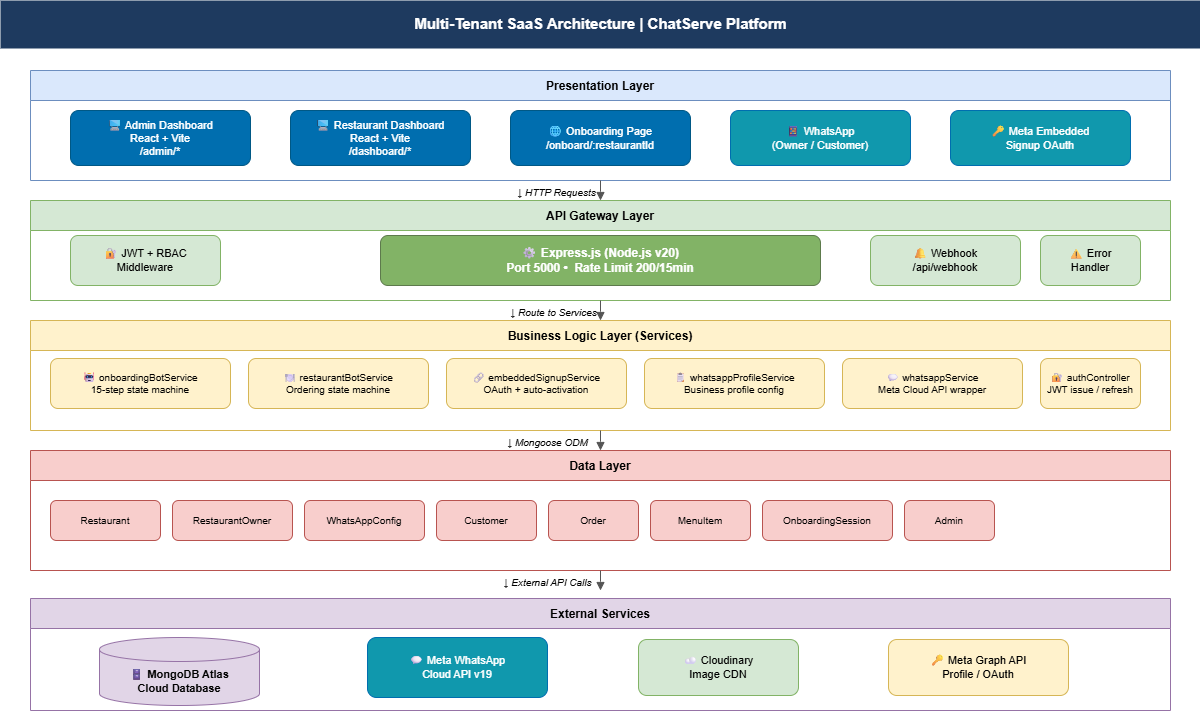
\includegraphics[width=0.99\textwidth]{Diagrams/system_architecture.png}
\caption{Overall System Architecture of ChatServe}
\label{fig:system_architecture}
\end{figure}

Above we present an architecture diagram which shows off the interaction between the frontend dashboards, Express.js backend, MongoDB database, and the Meta WhatsApp Cloud API. We see the message flow in through webhooks and are also show how various business tenants use the same back end infrastructure but at the same time have fully isolated data through the use of tenant scoped queries.


In a multi-tenant model we use a \textbf{shared database, shared schema} approach. Each data record for a business has a \texttt{business} ObjectId which is true for all of them and we at the API query level scope to the authenticated tenant's ID which is at the middleware layer. Thus we achieve full logical isolation between tenants at the same time we keep the infrastructure simple and cost effective.

\section{System Flow}

\subsection*{Business Onboarding Flow}

The business owner kicks off the onboarding process by sending the first message on WhatsApp. We have done away with the traditional form in favor of a guided chat which steps the user through the process. The bot puts out a series of questions which include the owner's name, business name, contact info, address, description, operating hours, business category, products or services and logo. As each response is received in real time they are stored which in turn improves accuracy and completeness.

\begin{figure}[H]
\centering
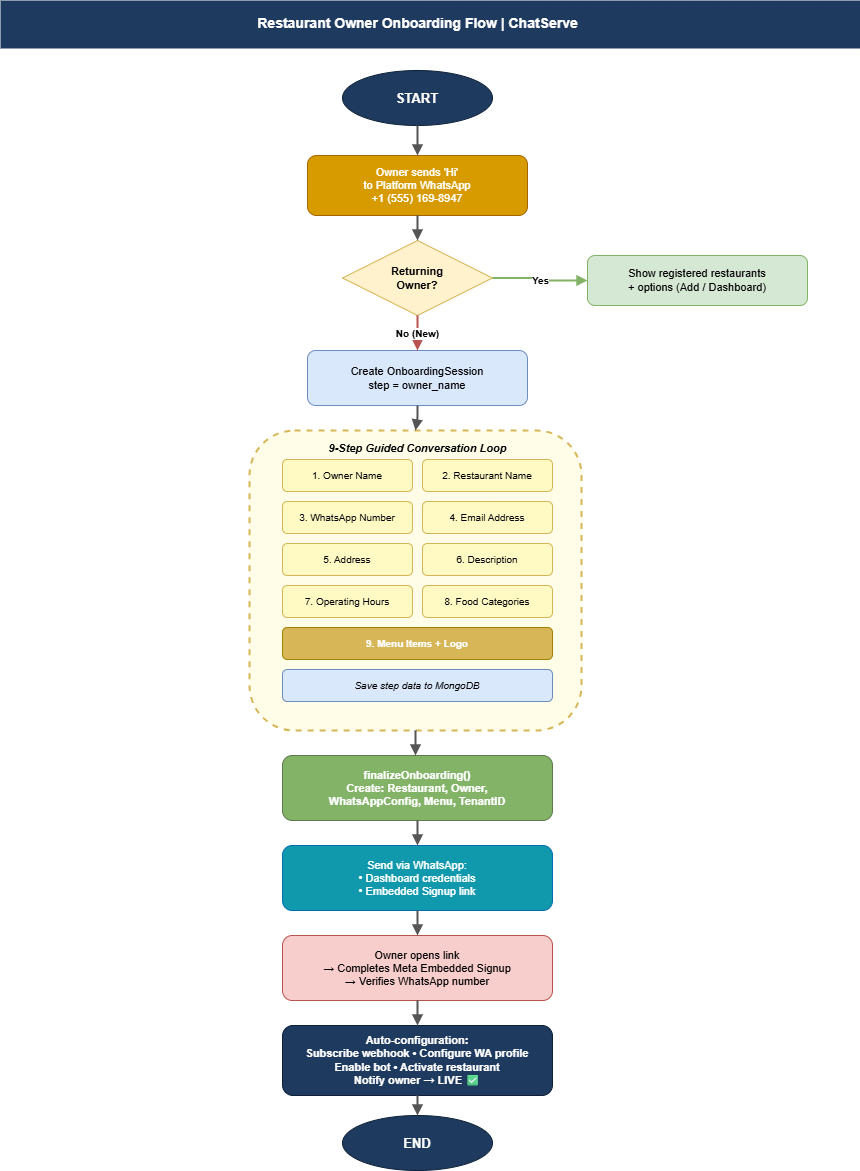
\includegraphics[width=0.85\textwidth]{Diagrams/Onboarding Flow.png}
\caption{Business Onboarding Flow via WhatsApp}
\label{fig:onboarding_flow}
\end{figure}

Once we have all the details we put together the required database records and we provide the owner a unique Embedded Signup link along to which they can access their dashboard also we give them login info. We have a very structured process in which each step is checked off before we move on to the next which in turn guarantees consistent and reliable data collection through out the onboarding.


\subsection*{Onboarding Sequence Diagram}
The diagram below shows in more detail the interaction between the business owner, the ChatServe backend, the MongoDB database, and the Meta WhatsApp Cloud API during the onboarding process. 

\begin{figure}[H]
\centering
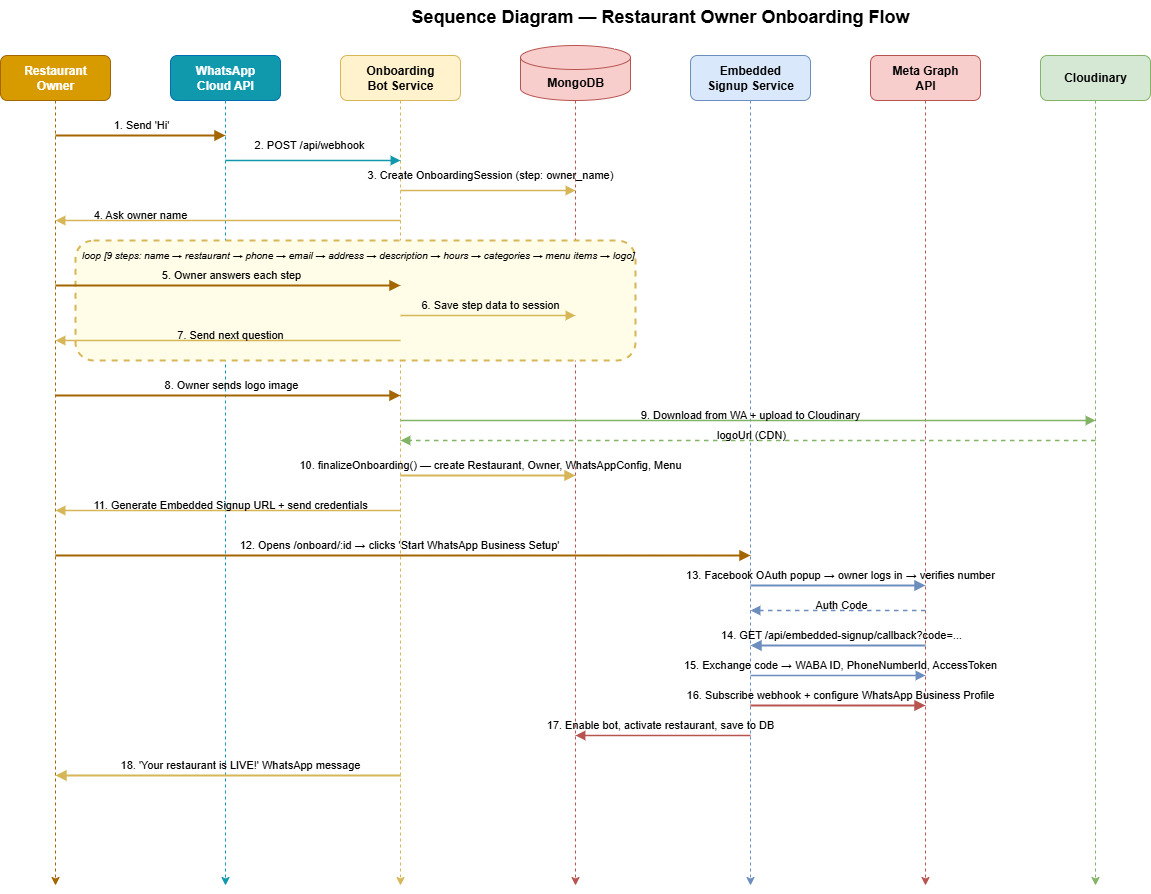
\includegraphics[width=0.99\textwidth]{Diagrams/Sequence_diagram - restauretn_Onboarding.png}
\caption{Sequence Diagram for Business Onboarding}
\label{fig:seq_onboarding}
\end{figure}

In the sequence diagram we see that each of owner's messages trigger a webhook POST to the backend. The backend which at this point is reading the present session state from MongoDB, determining the next move, out via the Meta API returns a response and also updates the session. This is a stateless request response cycle which plays out till we complete the tenth of the on boarding steps at which point the backend in question creates all tenant records and we dispatch the Embedded Signup link.

\subsection*{Customer Ordering Flow}

When a customer messages the business's WhatsApp number the webhook handler out of which the phone number is identified, we then go on to retrieve the customer and their session at the business, and the message is sent to the business bot. The bot in turn displays a very interactive main menu to the customer, allows them to look through categories and products or services, add what they like to a persistent cart, take them through a 3 step check out (address, confirm, pay) and at the end gives out an order confirmation message with a unique order ID. Also if the business owner updates any order status that change is immediately sent out to the customer via a WhatsApp message.

\subsection*{Customer Order Sequence Diagram}

\begin{figure}[H]
\centering
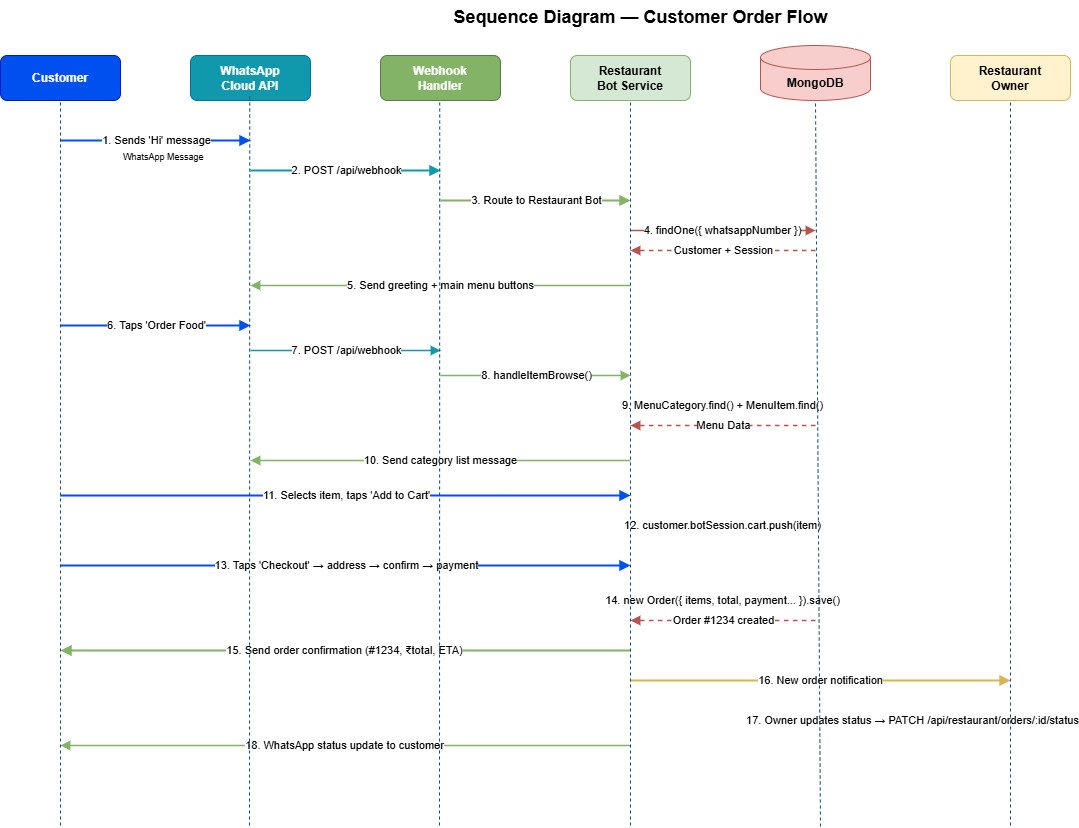
\includegraphics[width=0.90\textwidth]{Diagrams/Sequence_Diagram- cutomer_Order Flow.png}
\caption{Sequence Diagram for Customer Order Flow}
\label{fig:seq_ordering}
\end{figure}

The customer flow Sequence diagram which details the full message exchange from the time of the customer's first interaction through to the order confirmation. We see how the webhook routes messages to the proper business's bot, how we maintain the cart state between multiple exchanges, and how the final order is put into the database and reported back to the customer via WhatsApp.

\section{Database Design}

ChatServe uses MongoDB for it's primary data storage. We have designed the schema around the Business document which is our main focus. Also listed below are the key collections and their relationships.

\begin{figure}[H]
\centering
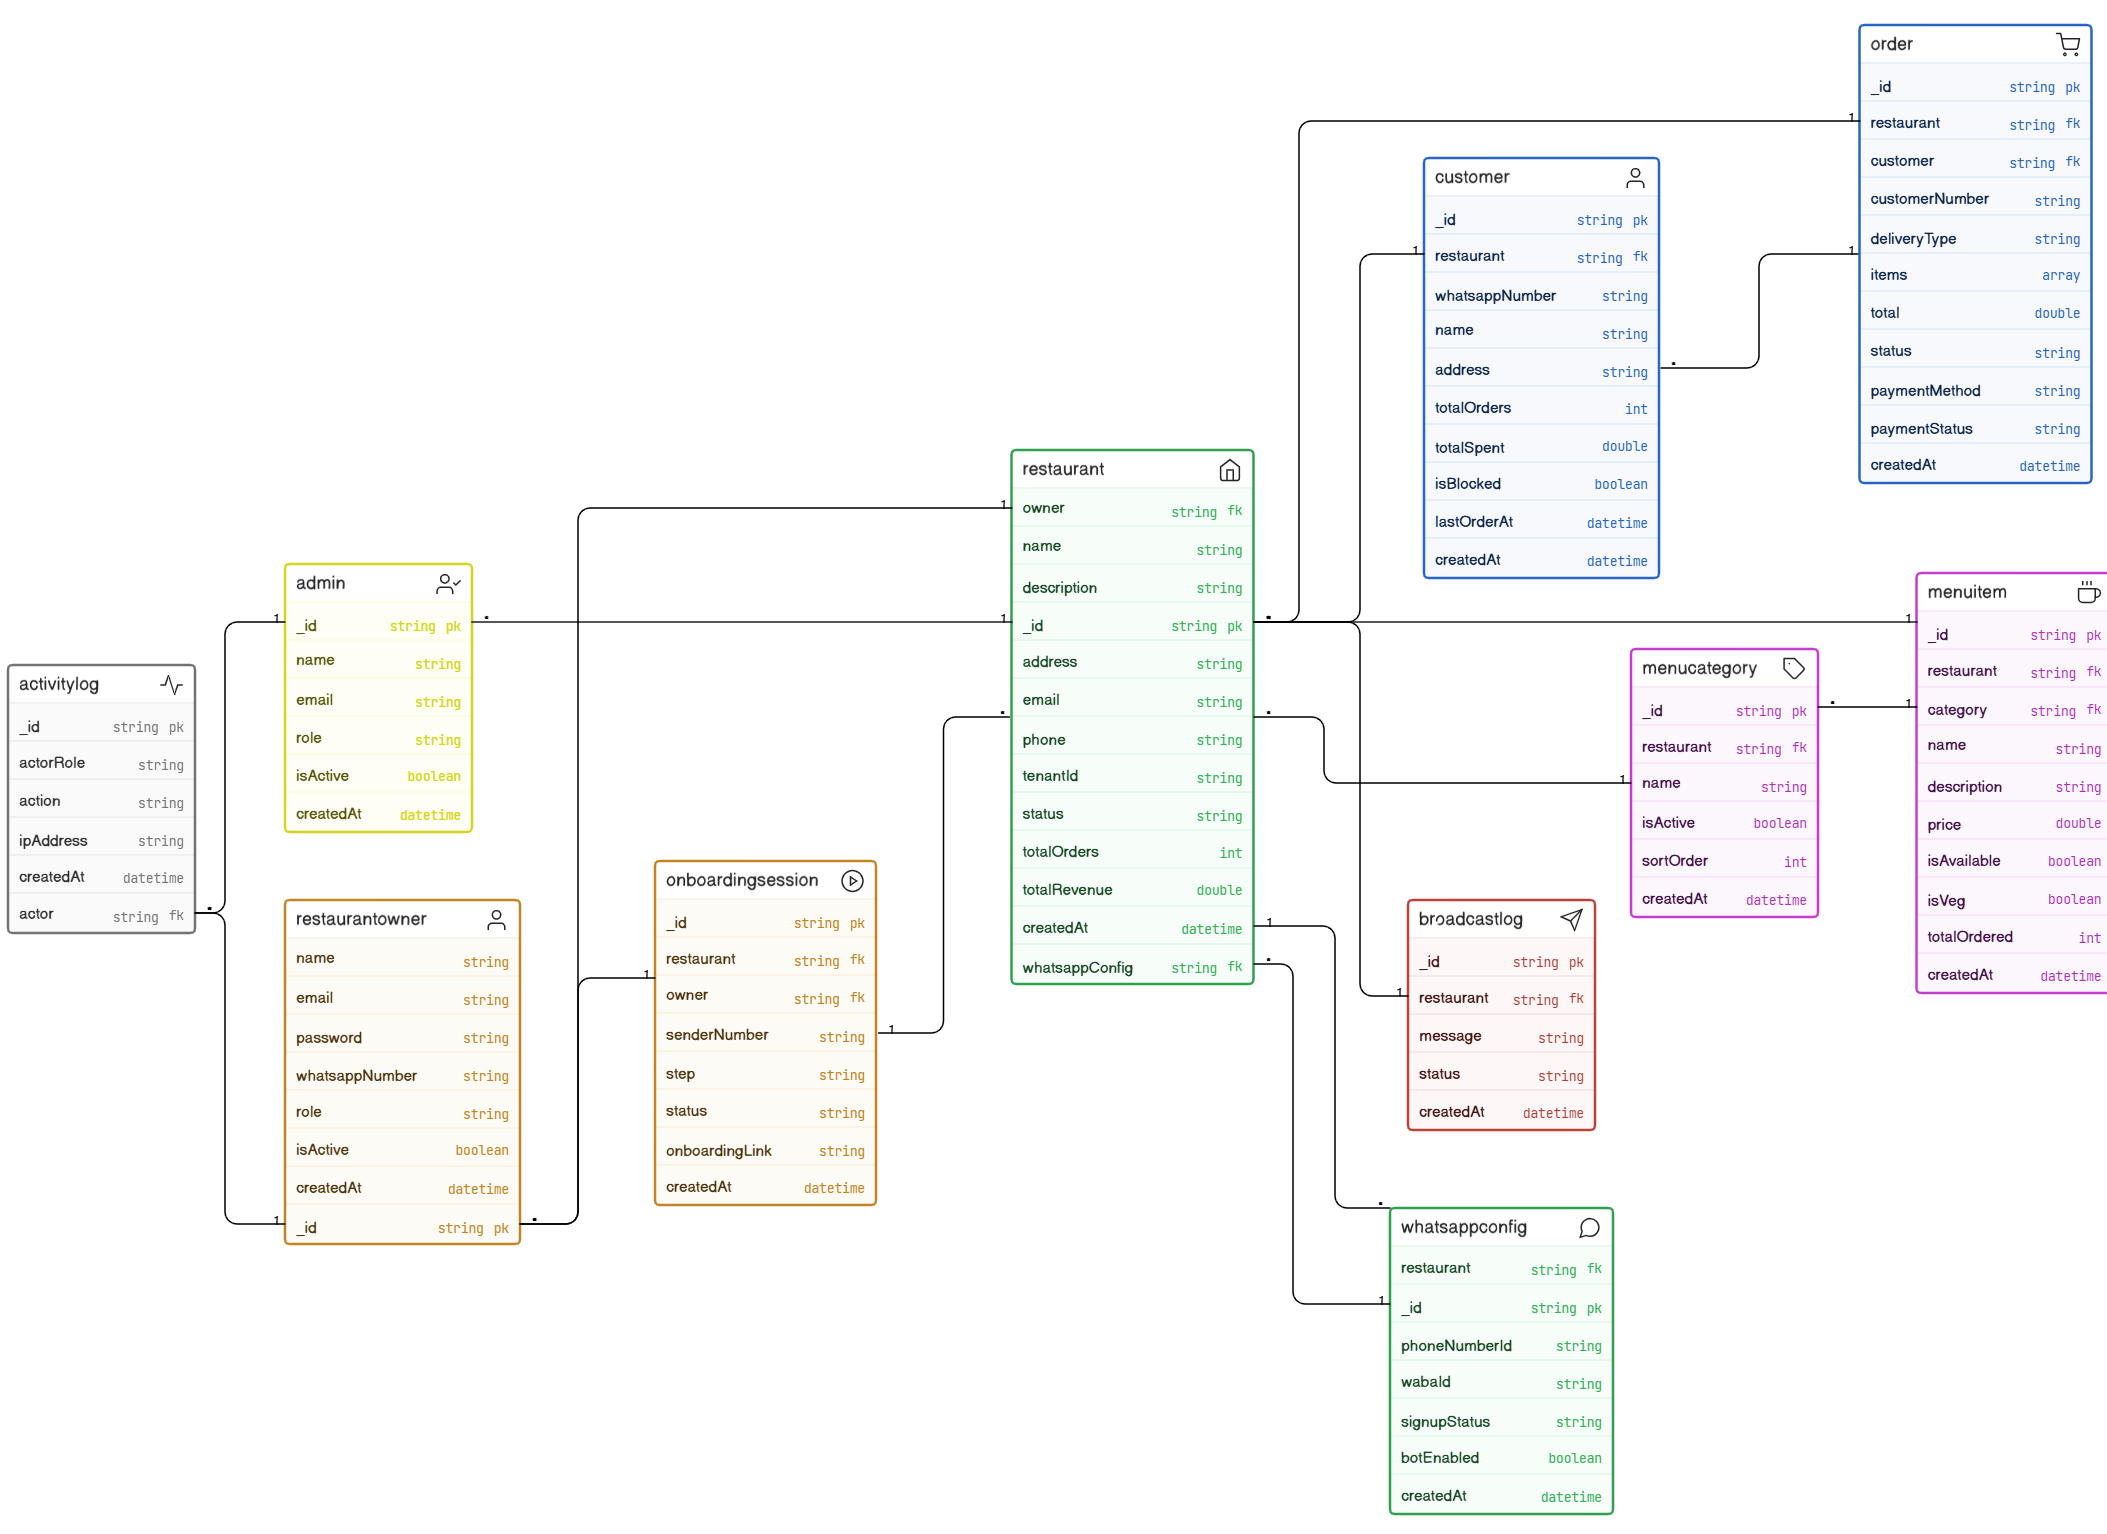
\includegraphics[width=0.99\textwidth]{Diagrams/er_diagram.png}
\caption{Entity-Relationship Diagram for the ChatServe Database}
\label{fig:er_diagram}
\end{figure}

In the diagram we present how each core collection interrelate which in turn serves as the root tenant for all other records. We have the WhatsAppConfig which puts in place Meta API credentials per business, Customer documents which we use for session and cart state and Order documents which cover the full order lifecycle. Also we use MongoDB ObjectIds for all foreign key references and have the businessId field indexed in each collection which in turn supports efficient tenant scoped queries.


\begin{itemize}

    \item \textbf{Business}: Core element document which includes business details, status, and which also puts forth all related collections.
    
    \item \textbf{BusinessOwner}: Auth info and contact details for the dashboard user.
    
    \item \textbf{WhatsAppConfig}: WABA ID, Phone Number ID, access token, webhook subscription status, and bot enable flag.
    
    \item \textbf{Customer}: Per each unique WhatsApp number per business we have the bot session state and cart.
    
    \item \textbf{CatalogItem}: Product/service catalog with pricing, category, availability and Cloudinary image URL.
    
    \item \textbf{Order}: Full order record including items, total, payment method, status and also a status history array.
    
    \item \textbf{OnboardingSession}: Goes over the registration progress of business owners which are in the process of on boarding.
    
    \item \textbf{Admin}: Platform admin credentials.

\end{itemize}

\begin{table}[H]
\centering
\caption{Core Collections and Key Fields}
\renewcommand{\arraystretch}{1.3}
\begin{tabularx}{\textwidth}{|l|X|}
\hline
\textbf{Collection} & \textbf{Key Fields} \\
\hline
businesses & name, status, tenantId, owner \\
\hline
whatsappconfigs & wabaId, phoneNumberId, botEnabled \\
\hline
customers & whatsappNumber, botSession, cart \\
\hline
orders & orderNumber, items, total, status \\
\hline
catalogitems & name, price, category, isAvailable \\
\hline
onboardingsessions & step, data, senderNumber \\
\hline
\end{tabularx}
\end{table}

\section{Implementation Details}

\subsection{Backend Implementation}

The backend is developed with Node.js and Express.js which we have structured into a modular architecture. This we did in order to put business logic at the charge of dedicated service layers from the route hander's perspective. In terms of the results we see enhanced maintainability and a better model of code organization.

\begin{lstlisting}[caption=Backend Directory Structure]
backend/
├── .env
├── .gitignore
├── config/
│   ├── cloudinary.js
│   ├── db.js
│   └── redis.js
├── controllers/
│   └── authController.js
├── middleware/
│   ├── auth.js
│   ├── errorHandler.js
│   └── upload.js
├── models/
│   ├── Admin.js
│   ├── Customer.js
│   ├── Logs.js
│   ├── Menu.js
│   ├── OnboardingSession.js
│   ├── Order.js
│   ├── Restaurant.js
│   ├── RestaurantOwner.js
│   └── WhatsAppConfig.js
├── package-lock.json
├── package.json
├── routes/
│   ├── admin.js
│   ├── analytics.js
│   ├── auth.js
│   ├── embeddedSignup.js
│   ├── menu.js
│   ├── onboarding.js
│   ├── order.js
│   ├── restaurant.js
│   ├── upload.js
│   └── webhook.js
├── server.js
├── services/
│   ├── emailService.js
│   ├── embeddedSignupService.js
│   ├── notificationService.js
│   ├── onboardingBotService.js
│   ├── restaurantBot/
│   │   ├── commands.js
│   │   ├── context.js
│   │   ├── index.js
│   │   ├── steps/
│   │   │   ├── cart.js
│   │   │   ├── checkout.js
│   │   │   ├── greeting.js
│   │   │   ├── help.js
│   │   │   ├── mainMenu.js
│   │   │   ├── menuBrowse.js
│   │   │   └── orders.js
│   │   └── utils/
│   │       └── messenger.js
│   ├── restaurantBotService.js
│   ├── whatsappProfileService.js
│   └── whatsappService.js
├── templates/
│   └── emails/
│       └── passwordReset.html
└── utils/
    ├── helpers.js
    ├── jwt.js
    ├── logger.js
    ├── phoneUtils.js
    └── seed.js

\end{lstlisting}

The chatbot modules present an approach which is state based, in that each user interaction is processed according to the current session state which is in MongoDB. Each incoming message sets off a state transition which in turn enables structured conversational flows like onboarding and order placement. We receive all WhatsApp messages via a webhook endpoint. The backend processes each request and routes it based on the associated phone number. At the platform level we have the onboarding bot which handles that traffic, at the business specific level we have separate ordering bots which do the processing, thus we achieve accurate handling in a multi tenant system.


\subsection{Frontend Implementation}

The frontend of our application is a React 18 Single Page Application which we built using Vite and we styled it with Tailwind CSS. We use TanStack Query for efficient server state management and caching.

\begin{lstlisting}[caption=Frontend Directory Structure, captionpos=b]
frontend/
├── .gitignore
├── index.html
├── package-lock.json
├── package.json
├── postcss.config.js
├── src/
│   ├── App.jsx
│   ├── components/
│   │   ├── PasswordResetModal.jsx
│   │   └── common/
│   │       └── StatCard.jsx
│   ├── context/
│   │   └── AuthContext.jsx
│   ├── index.css
│   ├── layouts/
│   │   ├── AdminLayout.jsx
│   │   └── RestaurantLayout.jsx
│   ├── main.jsx
│   ├── pages/
│   │   ├── admin/
│   │   │   ├── Broadcast.jsx
│   │   │   ├── Dashboard.jsx
│   │   │   ├── Onboarding.jsx
│   │   │   ├── RestaurantDetail.jsx
│   │   │   └── Restaurants.jsx
│   │   ├── auth/
│   │   │   ├── LoginPage.jsx
│   │   │   ├── OnboardError.jsx
│   │   │   ├── OnboardPage.jsx
│   │   │   └── OnboardSuccess.jsx
│   │   └── restaurant/
│   │       ├── Broadcast.jsx
│   │       ├── Customers.jsx
│   │       ├── Dashboard.jsx
│   │       ├── Menu.jsx
│   │       ├── Orders.jsx
│   │       ├── Profile.jsx
│   │       └── WhatsApp.jsx
│   └── services/
│       └── api.js
├── tailwind.config.js
└── vite.config.js

\end{lstlisting}

The application has role based designs for Admin and Business Owner users. We use JWT tokens for authentication. Access tokens are of 15 minute duration and issue refresh tokens which are valid for 7 days. We include auth headers in API requests and we have put in place a silent token refresh which takes care of expired sessions thus providing a smooth user experience.


\section{System Features and Functionalities}

The presented system reports an extensive set of features which we put forward for business onboarding, order and booking management, and customer interaction via WhatsApp.

\begin{itemize}

\item \textbf{Platform Onboarding Bot:}
A chatbot that walks business owners through a series of steps in the registration process on WhatsApp. It supports text input, image upload, session management, and the auto creation of required database entries. At the end we provide login info to the owner.

\item \textbf{Meta Embedded Signup Integration:}
Enables the business to connect with WhatsApp Business API which is a service of Meta via our OAuth based Embedded Signup flow. We auto fill in the required info and take care of backend config which includes setting up webhooks and activating the bot.

\item \textbf{Automatic WhatsApp Business Profile Configuration:}
Automatically maintains the business's WhatsApp Business profile via Meta Graph API. We sync business name, description, category, and contact info with the platform data.

\item \textbf{Business Ordering Bot:}
An interactive chatbot that which customers use to go through product or service categories, see available offerings, put things in their cart, and place orders. We have a structured checkout process and also we which remember customer context for return users.

\item \textbf{Business Owner Dashboard:}
A web based platform which includes key functions of order management, product/service catalog update, customer tracking, and basic analytics which in turn includes order trends, and revenue reports.

\item \textbf{Super Admin Dashboard:}
Centralized to all aspects of the platform which includes business management, onboarding, monitoring, system configuration, and broadcast communication with business owners.

\end{itemize}


\section{Results}

Screenshots illustrating the complete functionality of the created platform are provided below for each of the three user types.

\begin{figure}[H]
\centering
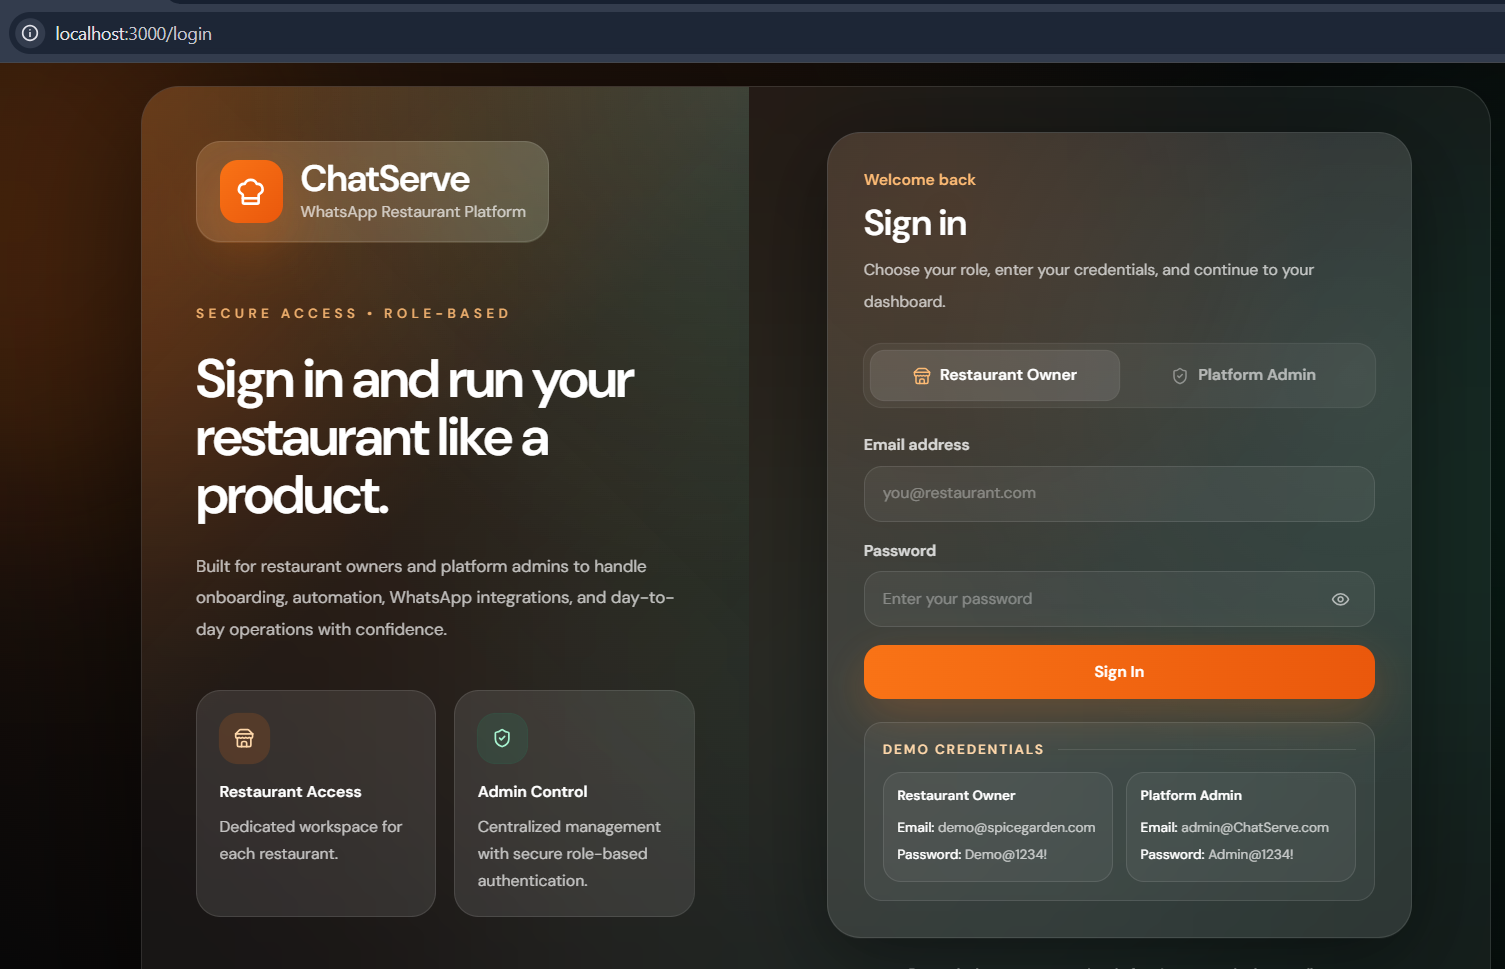
\includegraphics[width=0.80\textwidth]{Diagrams/loginpage.png}
\caption{Login Page for Super Admin and Business Owner}
\label{fig:login}
\end{figure}

The login page provides role-based authentication that directs admins to the Super Admin dashboard and business owners to their personal account page. The session is protected by the JWT mechanism, with access tokens expiring after 15 minutes and refreshing after 7 days.

\subsection{Business Registration via WhatsApp}
Below you can see the actual WhatsApp conversation between a business owner and the bot guiding the latter in the registration process. The bot asks all the necessary questions, and the owner just needs to answer them.

\begin{figure}[H]
\centering
\begin{minipage}{0.48\textwidth}
    \centering
    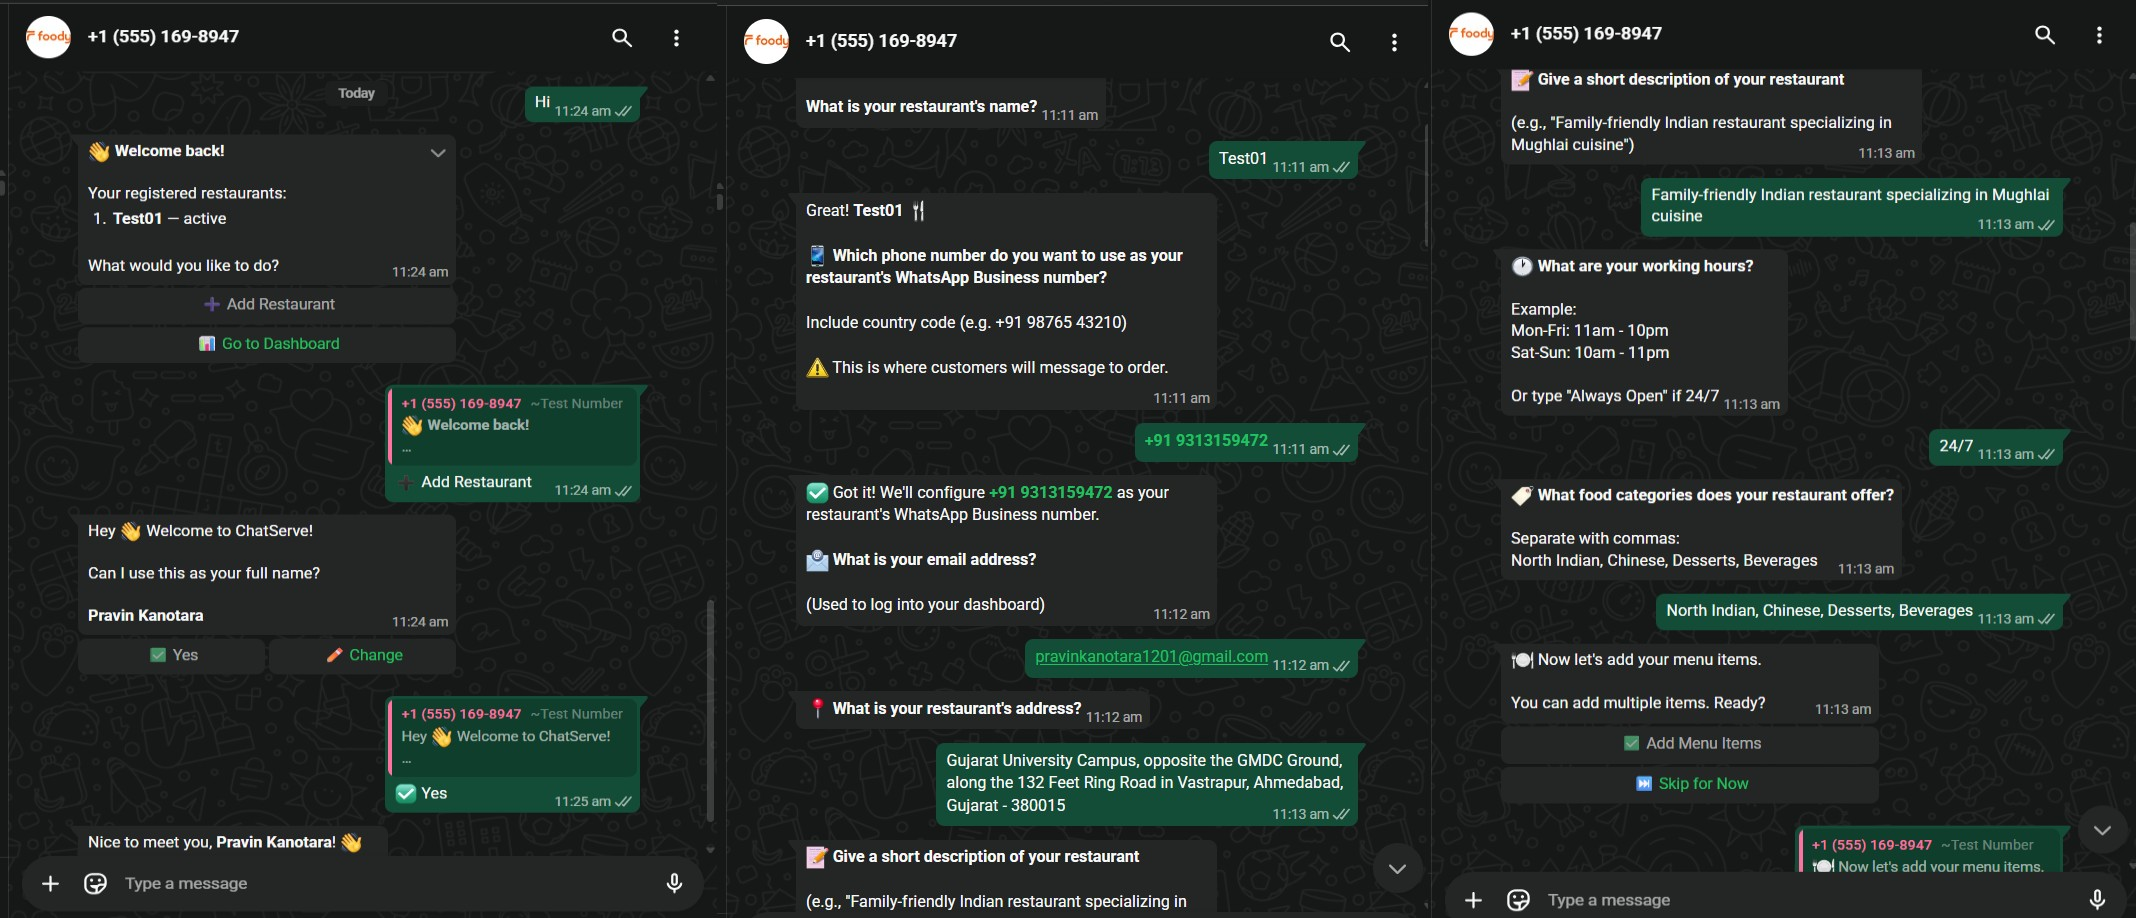
\includegraphics[width=\linewidth]{Diagrams/restaurant_reg1_3.jpg}
    \caption*{(a) Steps 1-3: Owner's name, business name, WhatsApp number}
\end{minipage}
\hfill
\begin{minipage}{0.48\textwidth}
    \centering
    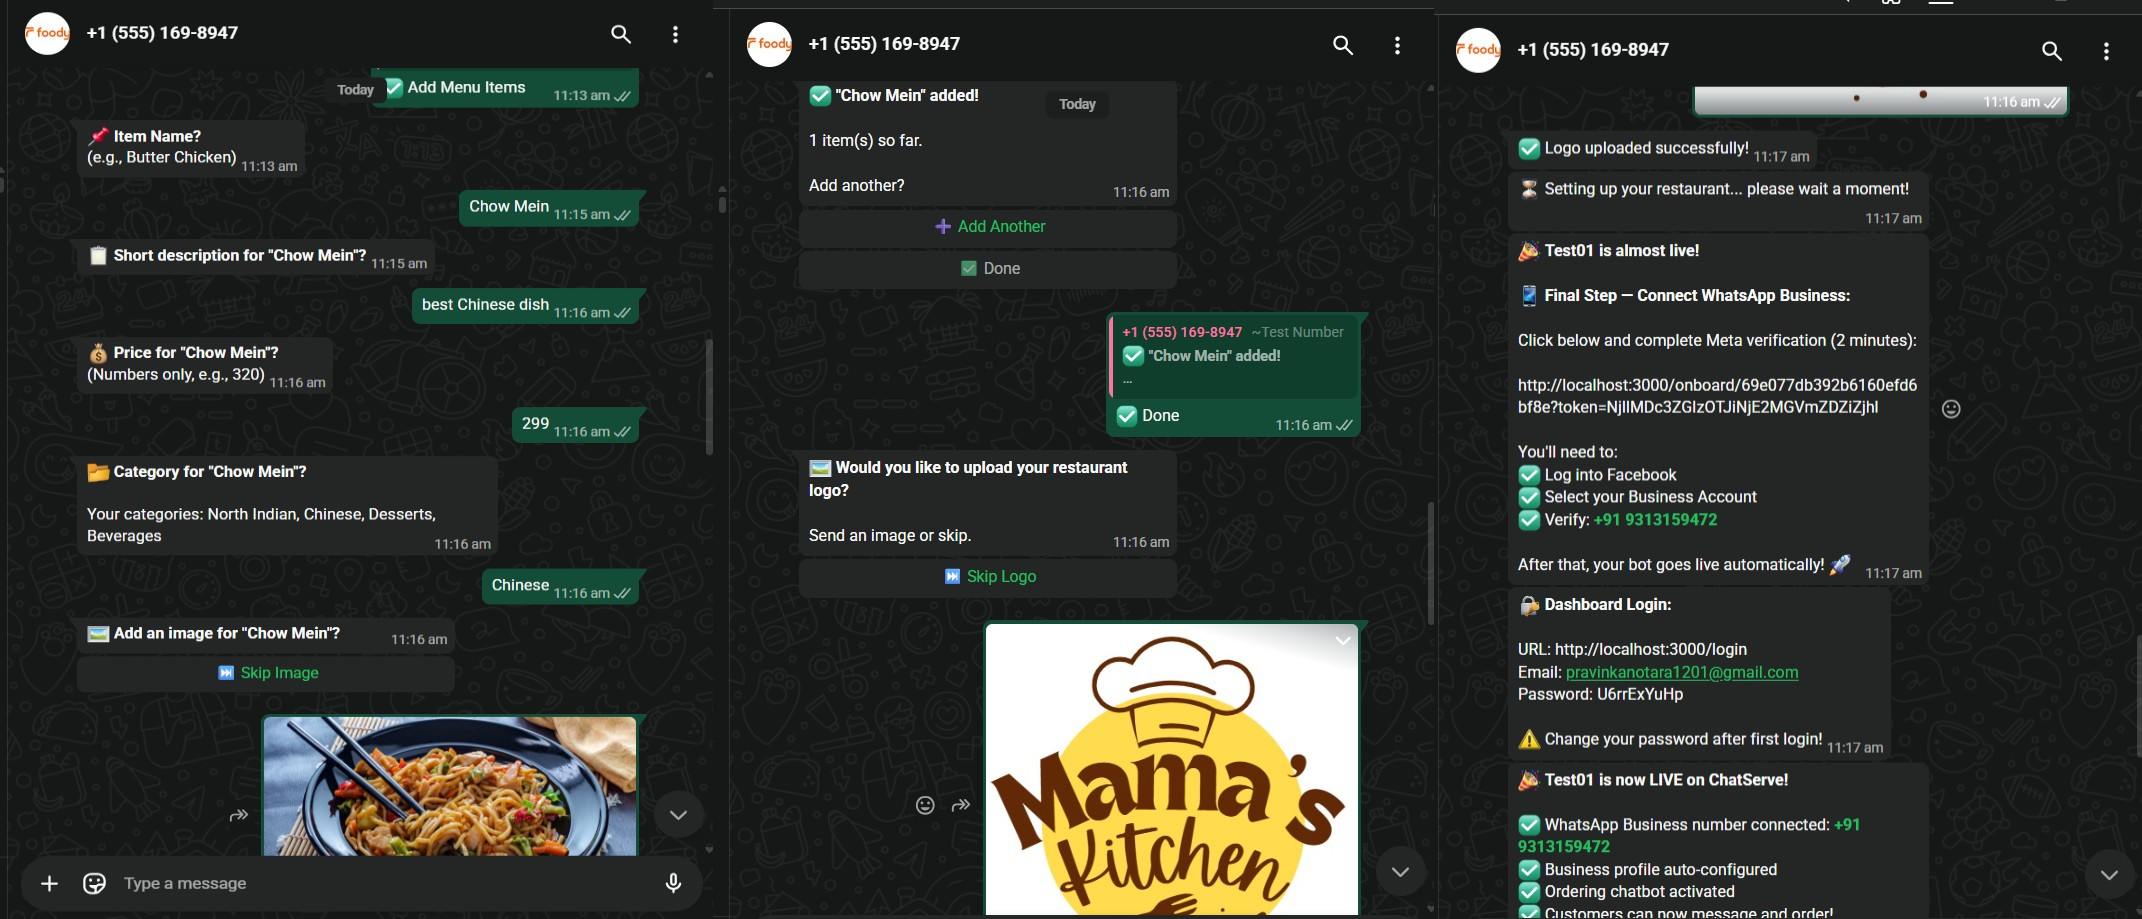
\includegraphics[width=\linewidth]{Diagrams/restaurant_reg_4_6.jpg}
    \caption*{(b) Steps 4-6: Email address, business address, description}
\end{minipage}
\caption{Actual WhatsApp Onboarding Process for Business Owners}
\label{fig:wa_registration}
\end{figure}

From the above, it becomes clear that the onboarding process is fully conversational and is carried out completely inside WhatsApp messenger. Furthermore, every question posed by the bot to the business owner gets validated, and the bot will repeat itself in case of an invalid response.

\subsection{Admin Dashboard and Controls}

\begin{figure}[H]
\centering
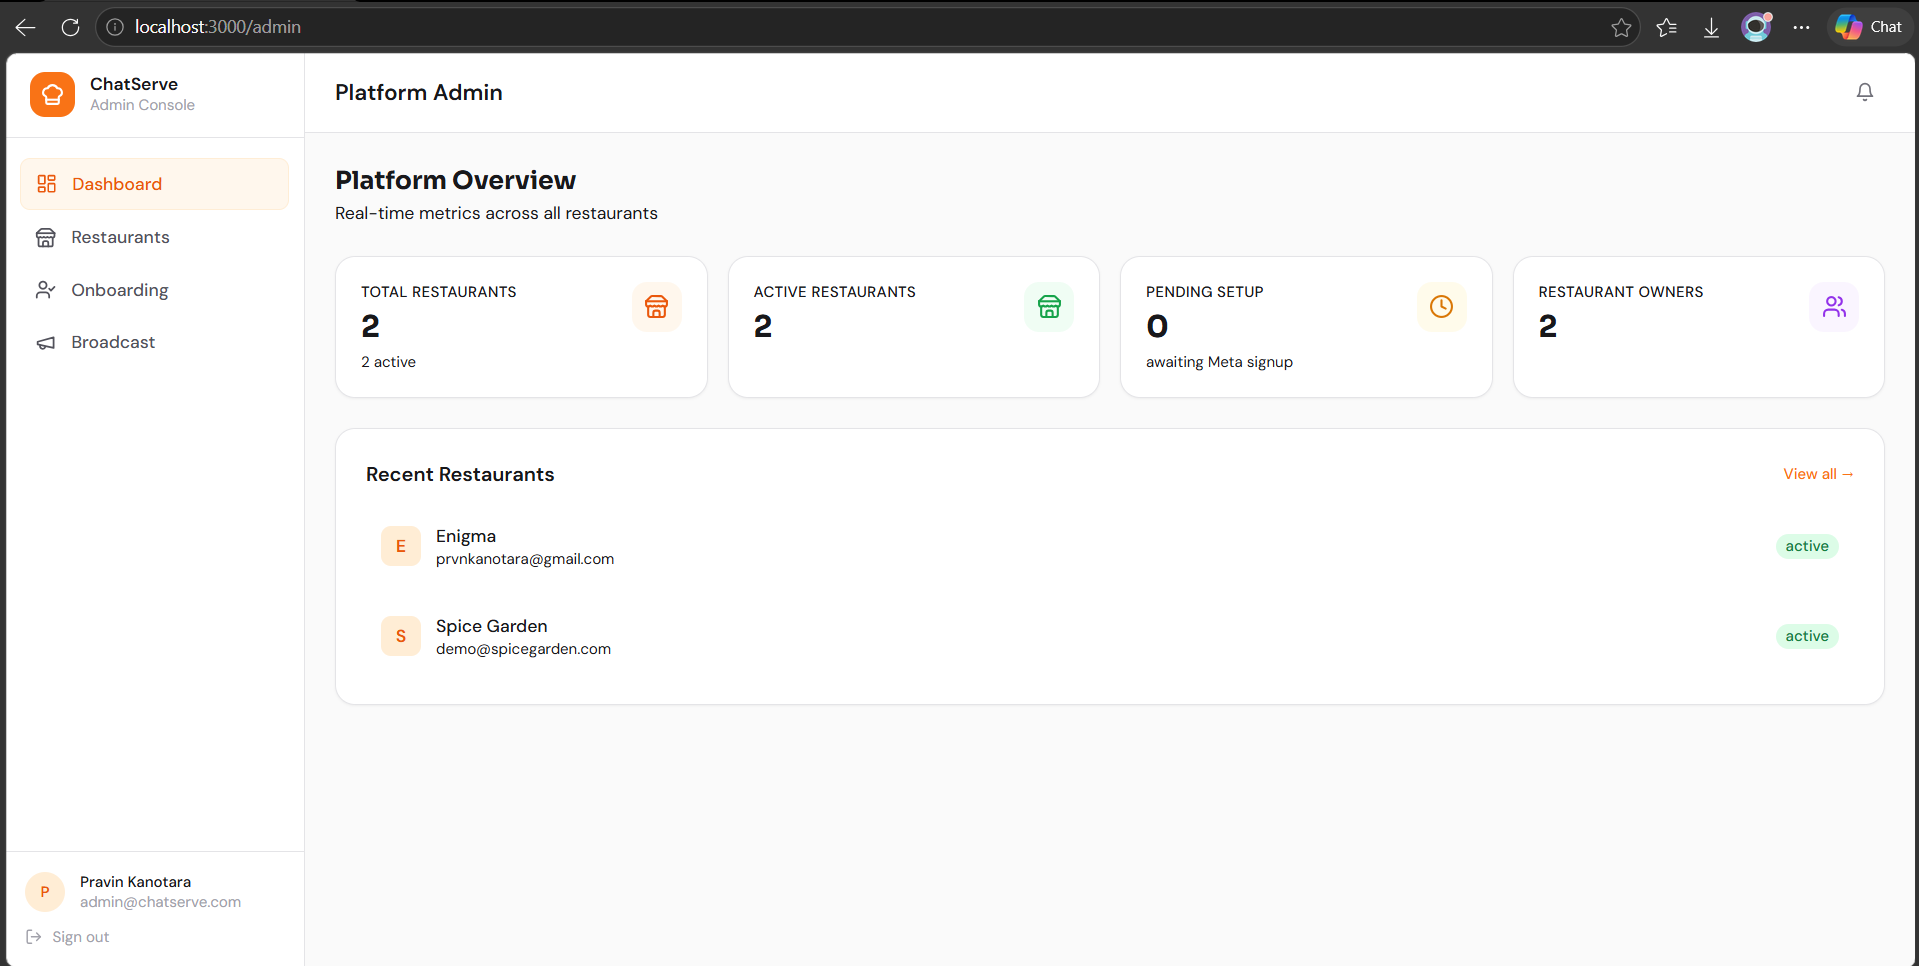
\includegraphics[width=0.95\textwidth]{Diagrams/admin_dashboard .png}
\caption{Admin Dashboard: Platform KPIs Overview and Businesses Listing}
\label{fig:admin_dashboard}
\end{figure}

The administrator sees a general overview of all activities occurring within the platform. It includes KPIs like the total number of registered businesses, active bots, order count and other metrics. Furthermore, it is possible to open a detailed view for each individual business to either activate/deactivate it or to configure its WhatsApp integration.

\begin{figure}[H]
\centering
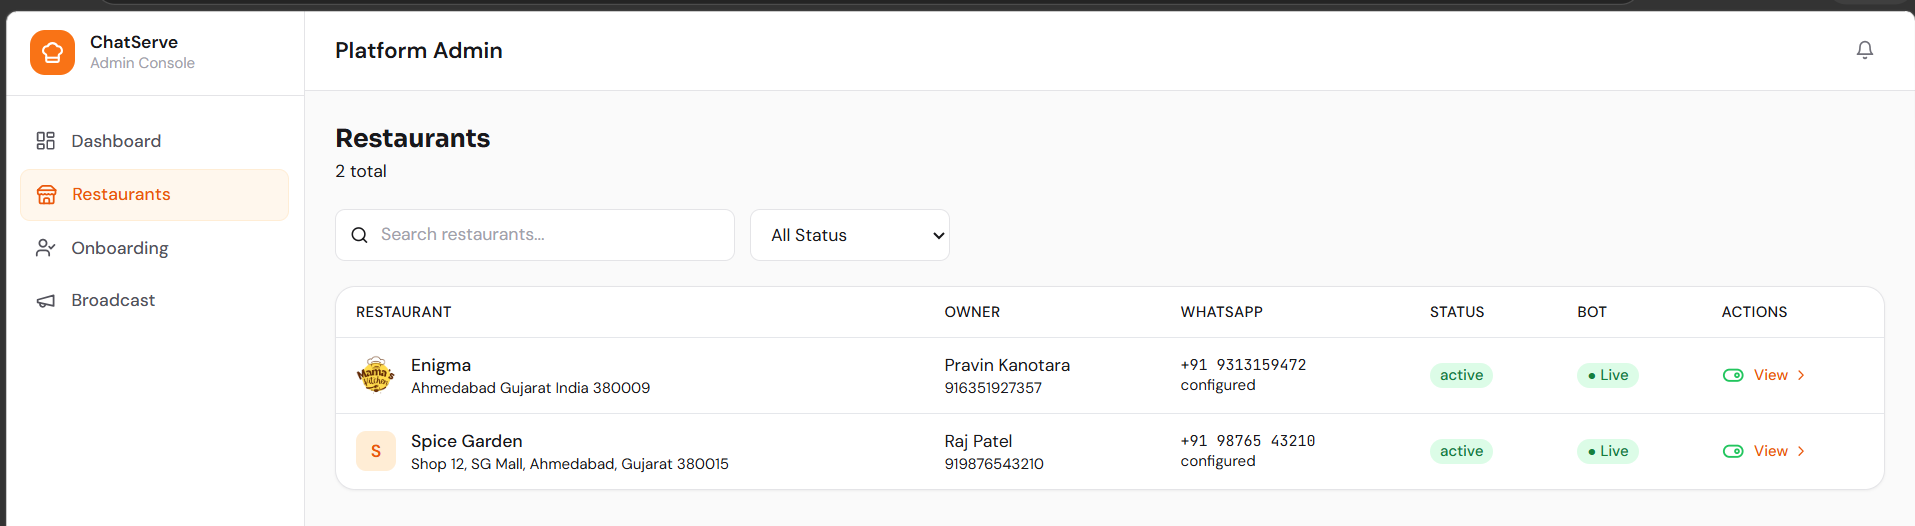
\includegraphics[width=0.95\textwidth]{Diagrams/admin_restaurents.png}
\caption{Listing of Registered Businesses on Admin Interface}
\label{fig:admin_restaurants}
\end{figure}

Here the business is presented in the list along with its current activation status (pending, active or suspended). It also has an icon that allows opening a page with detailed settings for that business or manually activating/deactivating its WhatsApp configuration.

\begin{figure}[H]
\centering
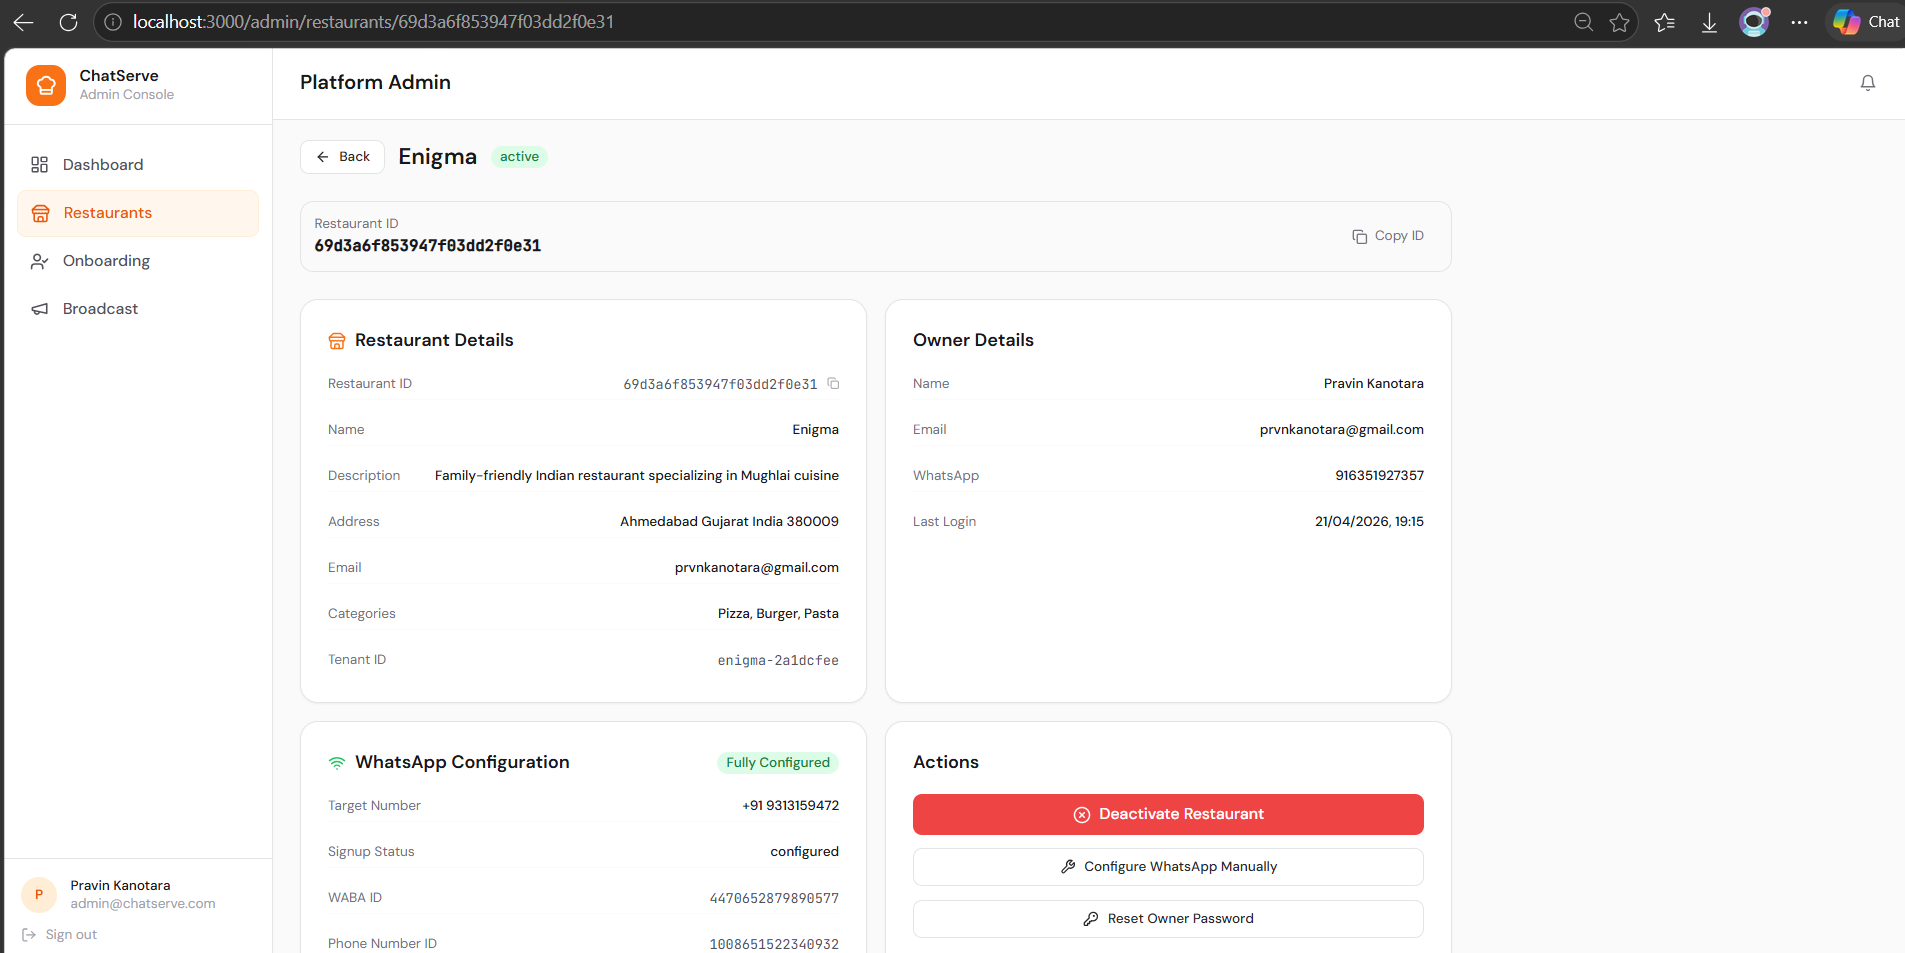
\includegraphics[width=0.95\textwidth]{Diagrams/admin_restaurent_details.png}
\caption{Detailed Information about a Business}
\label{fig:admin_restaurant_detail}
\end{figure}

As seen from above, the business detail view provides an administrator with important information such as WhatsApp Business Account ID, Phone Number ID, webhook endpoint validation status, and status of its bot. In addition, the administrator can use the ``manual setup'' block to populate WhatsApp integration information manually.

\begin{figure}[H]
\centering
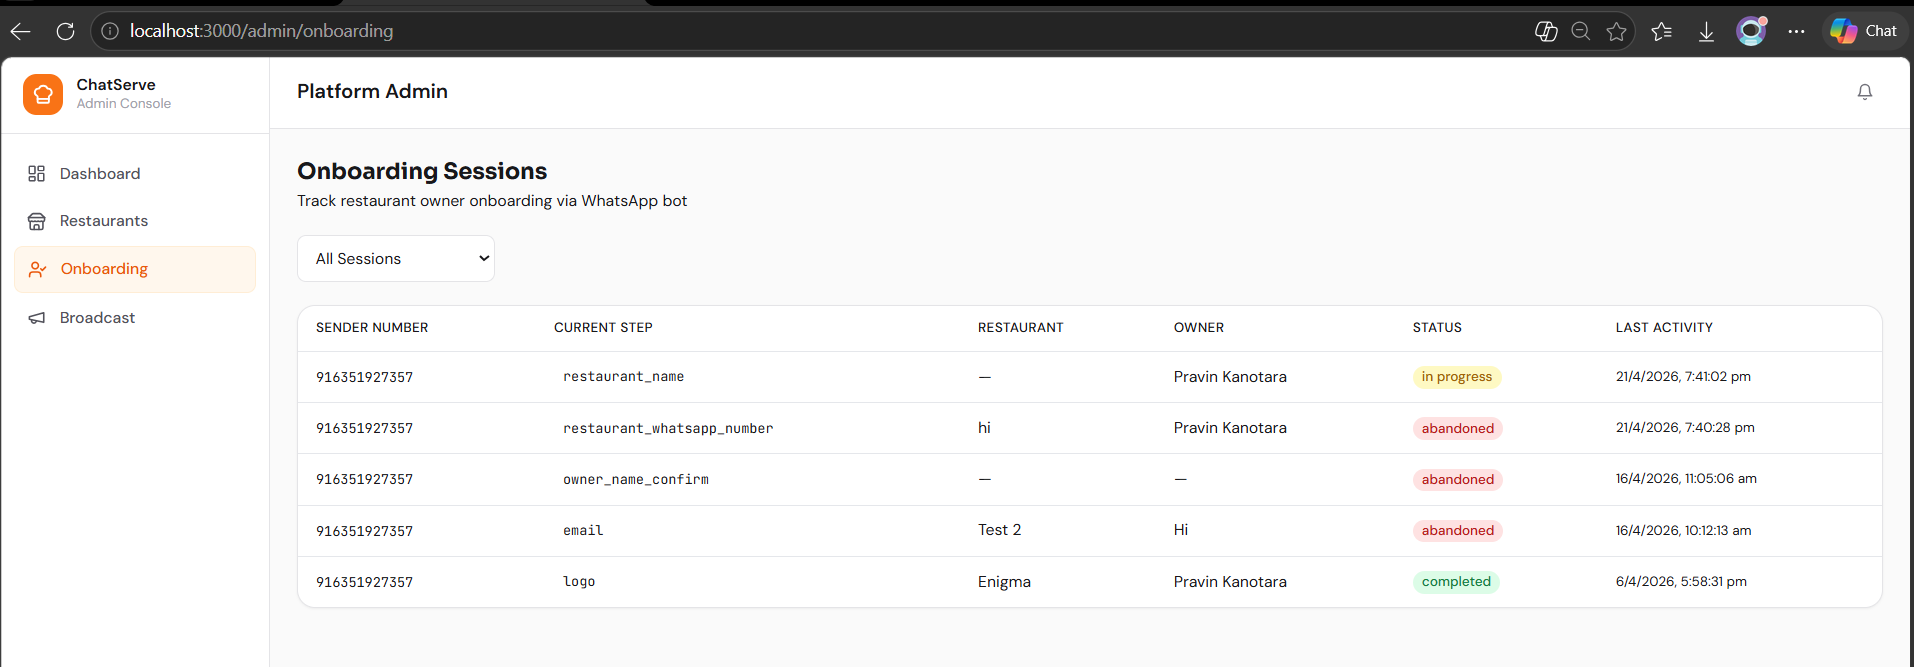
\includegraphics[width=0.95\textwidth]{Diagrams/admin_onboarding.png}
\caption{Dashboard: Ongoing Onboarding Sessions Monitor}
\label{fig:admin_onboarding}
\end{figure}

Here the platform administrator has live monitoring of all ongoing onboarding processes. For each ongoing session the administrator knows the WhatsApp number of the sender, the question number they are at now and the time when the session started.

\begin{figure}[H]
\centering
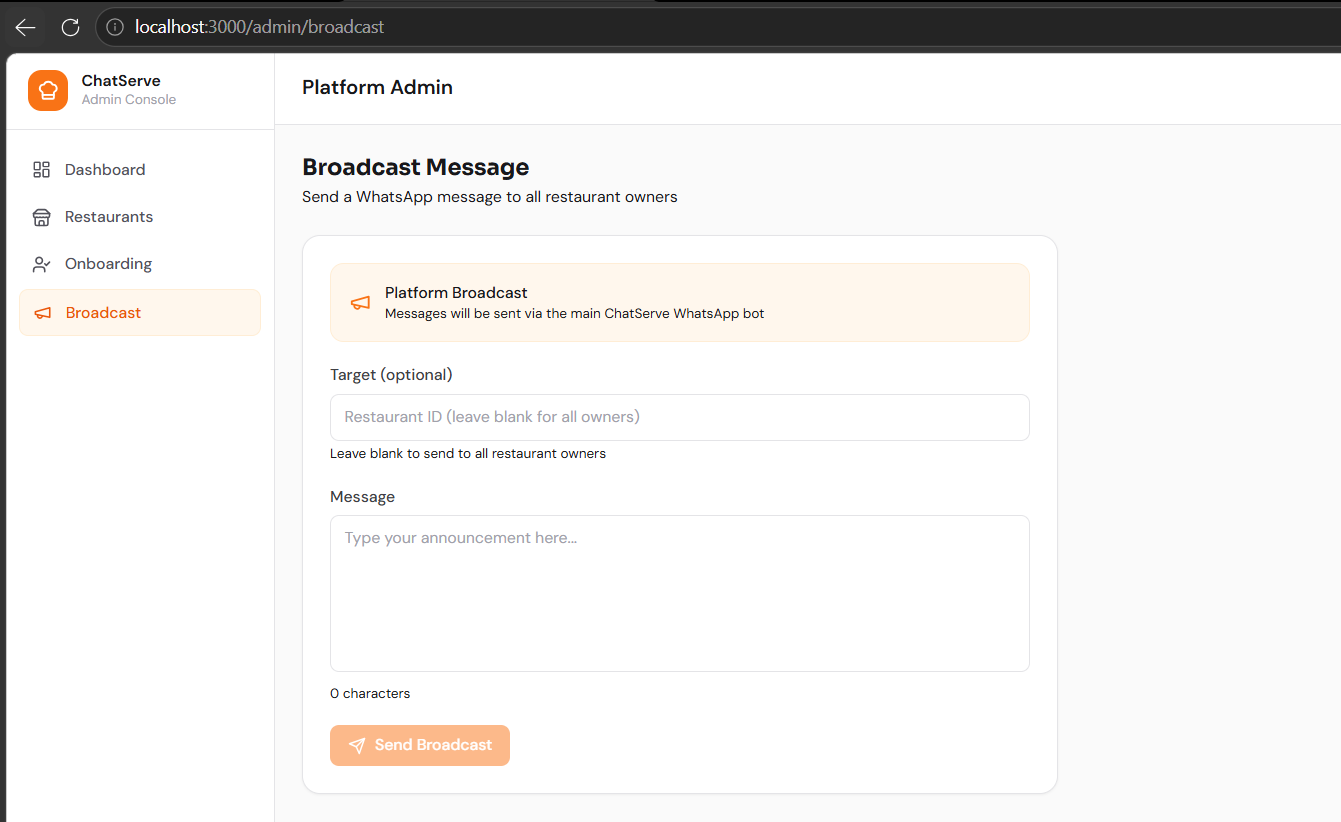
\includegraphics[width=0.95\textwidth]{Diagrams/admin_brodcast.png}
\caption{Administrator Broadcast Messaging Module}
\label{fig:admin_broadcast}
\end{figure}

The administrator can broadcast messages to all owners of registered businesses at once by using this module. The message would get sent to the owner's WhatsApp number via the Meta Cloud API.

% ── Business Owner Dashboard ───────────────────────────────────────────────
\subsection{Business Owner Dashboard}

\begin{figure}[H]
\centering
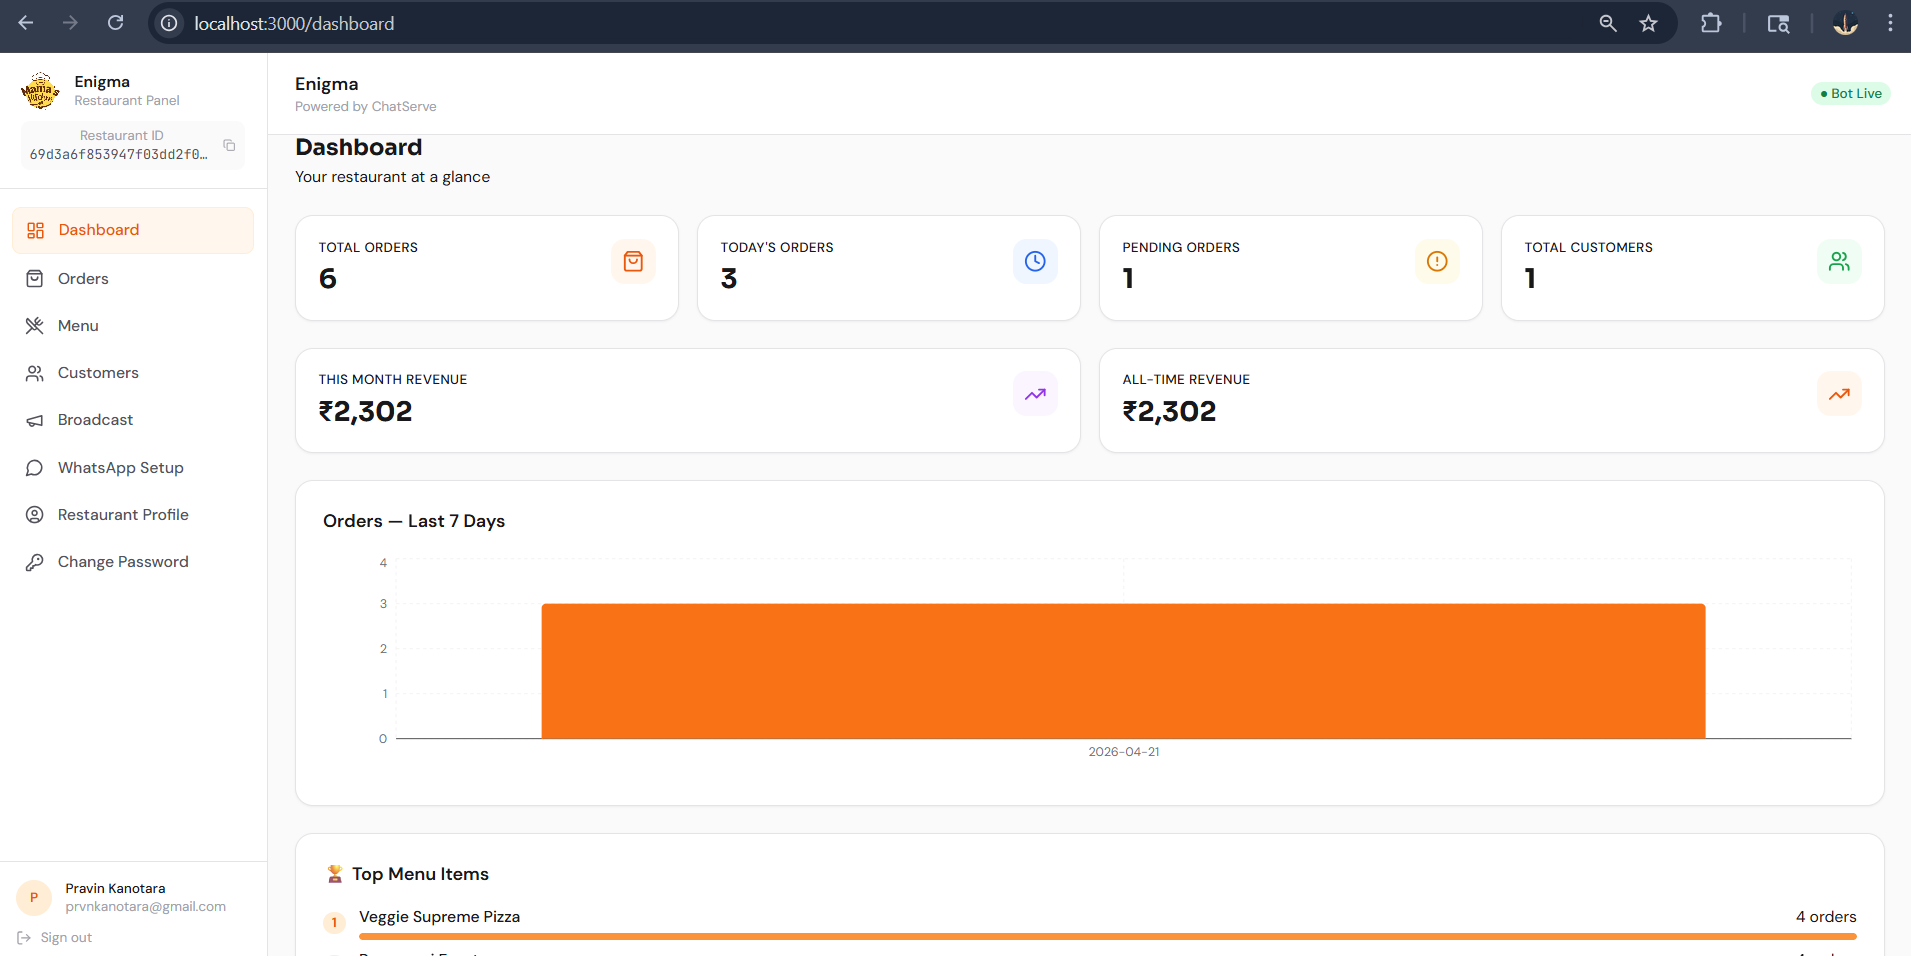
\includegraphics[width=0.95\textwidth]{Diagrams/restaurant_dashboard.png}
\caption{Business Owner Dashboard: Orders Today}
\label{fig:restaurant_dashboard}
\end{figure}

Business owners see general statistics for the day in the upper part of the screen, including the total number of orders, earned money and unique customers. Moreover, a seven-day chart showing the evolution of orders is presented here. Lastly, below that owners see the list of the orders of the day.

% ── Catalog Management ──────────────────────────────────────────────────────
\begin{figure}[H]
\centering
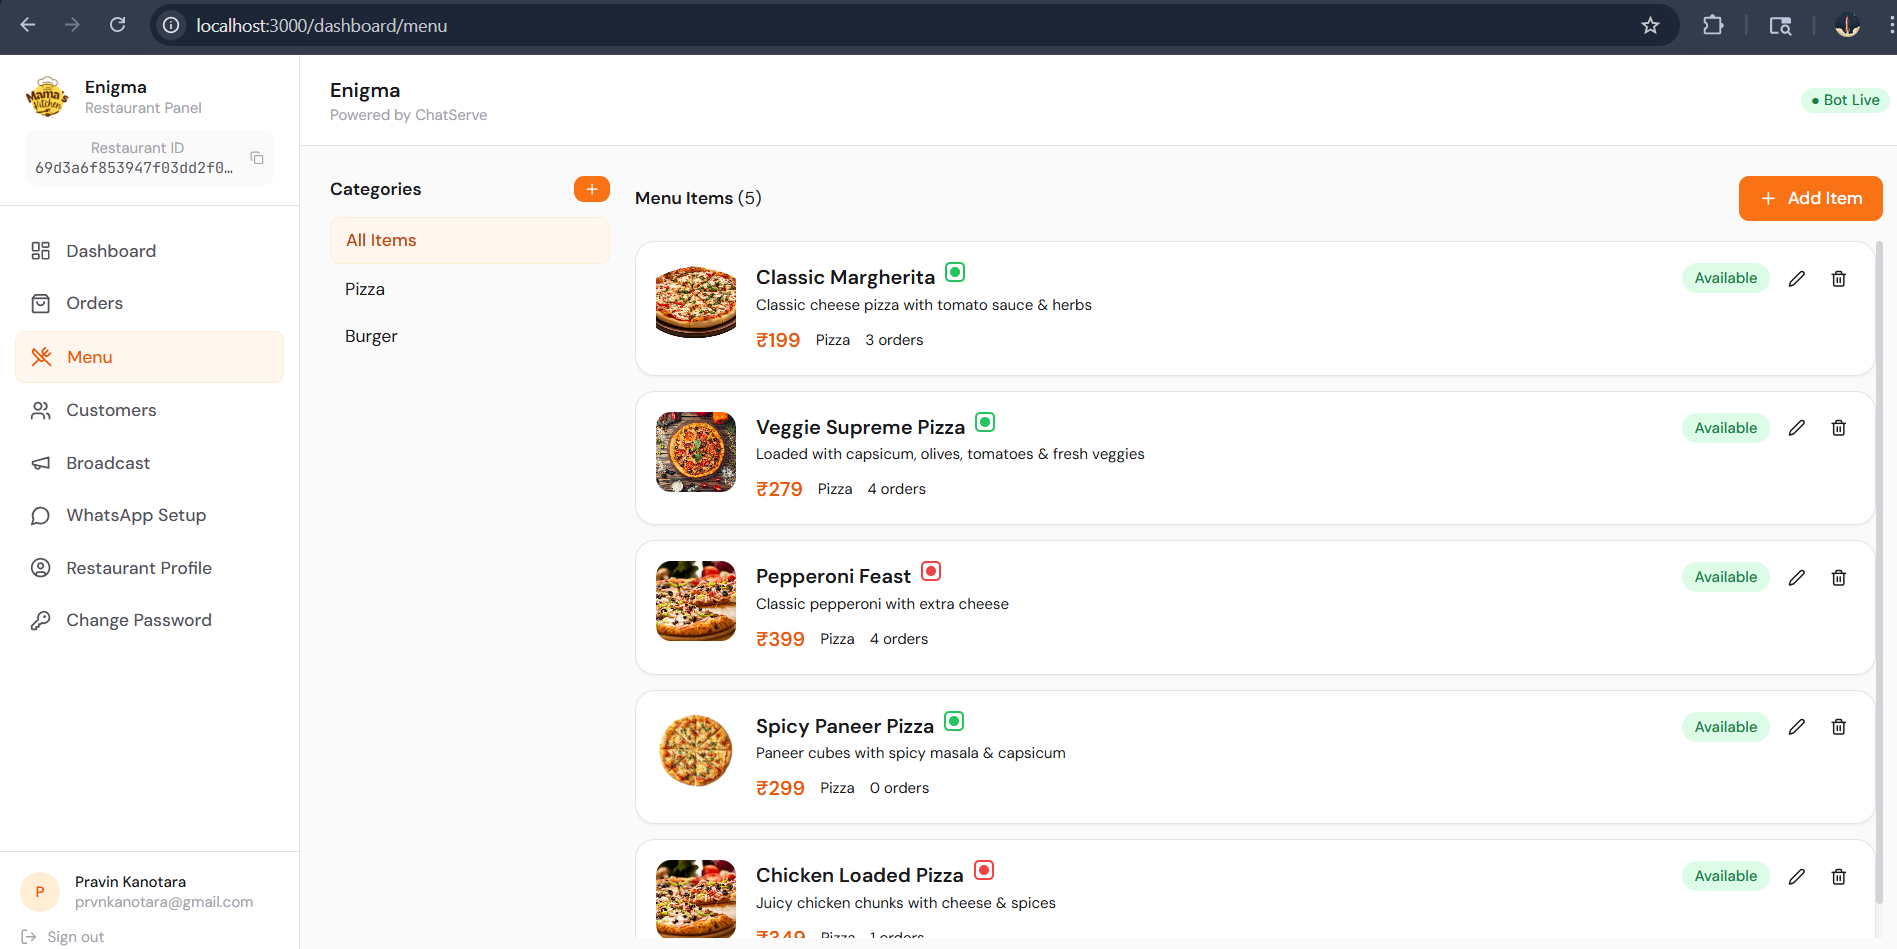
\includegraphics[width=0.95\textwidth]{Diagrams/restaurant_menu.png}
\caption{Product/Service Catalog Management Module}
\label{fig:menu_management}
\end{figure}

Catalog management allows business owners to view all products or services divided into categories. Here we can see the item name, price and status (currently active or disabled). In addition, the owner can toggle the item's status, thus changing the behavior of the bot when responding to user queries. Lastly, there is an opportunity to add new items by filling out a simple form (accessible by clicking the appropriate button).

% ── WhatsApp Business Profile ─────────────────────────────────────────────────
\begin{figure}[H]
\centering
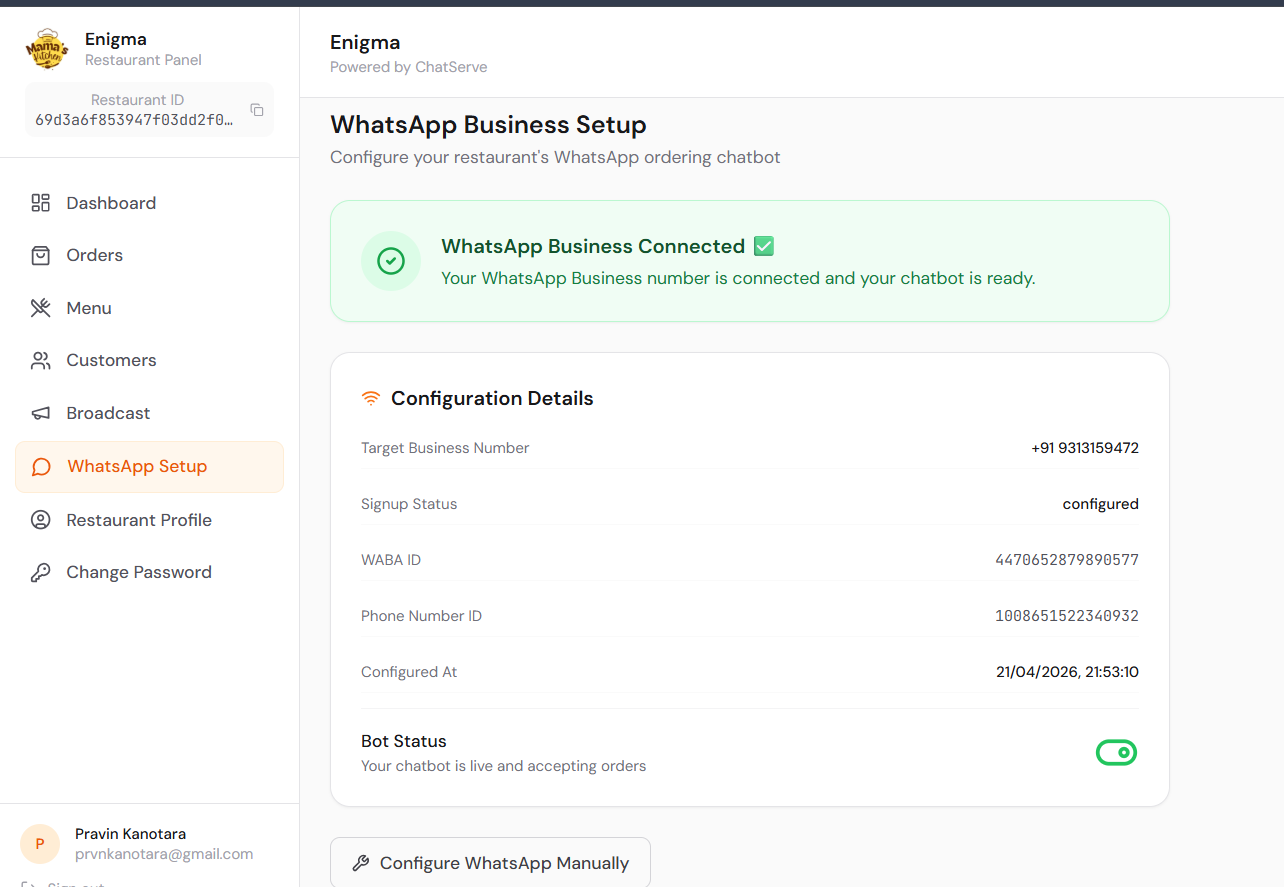
\includegraphics[width=0.85\textwidth]{Diagrams/restaurant_WAprofile.png}
\caption{Business's Auto-Configured WhatsApp Business Profile}
\label{fig:wa_profile}
\end{figure}

Below we see the automatically configured WhatsApp Business Profile of one of our businesses. It should be noted that all the data presented here was automatically populated based on the information provided by the owner during the onboarding conversation.

% ── Business Broadcast ──────────────────────────────────────────────────────
\begin{figure}[H]
\centering
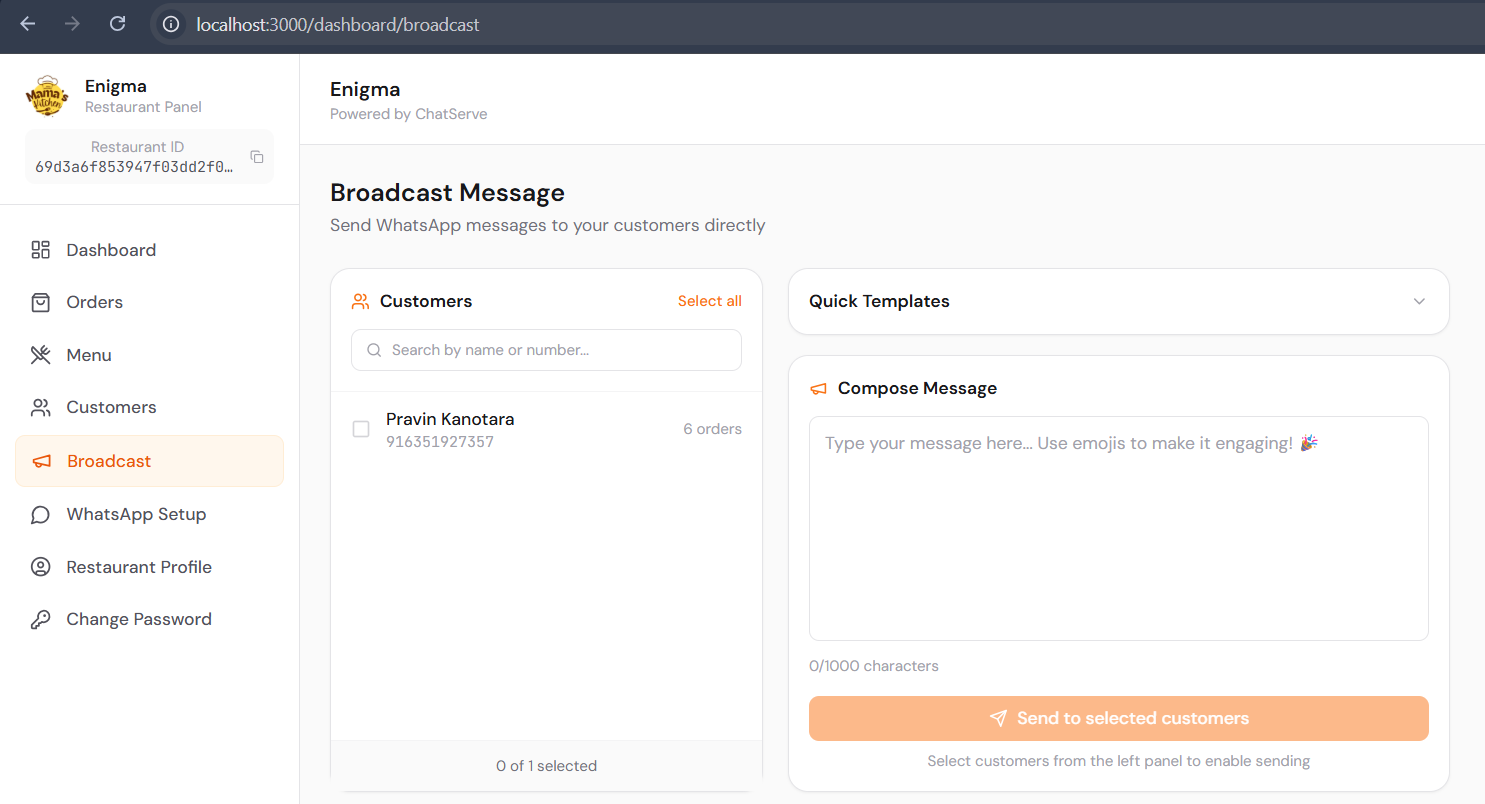
\includegraphics[width=0.95\textwidth]{Diagrams/restaurant_brodcast.png}
\caption{Business Owner's Broadcast Module}
\label{fig:restaurant_broadcast}
\end{figure}

Finally, the business owner can broadcast his own message to his customers using this module. The message would get delivered to all those customers who interacted with the business bot before.




\section{Discussion}

\subsection{Functionality Verification}

The system complies with all functional requirements, namely: business integration, WhatsApp ordering, and dashboard management. In general, the whole process of customer engagement to order confirmation works as expected.

\subsection{System Behavior}

Formal system testing could not be performed because of the lack of a production environment. But based on development and system usage, the system exhibited stable behavior for key functionalities, such as authentication, data processing, and bot messaging.

\subsection{System Design Issues}

Multi-tenant architecture allows logical data separation between different business accounts. Additionally, the system can configure automatically the WhatsApp Business Profile, including the use of the Embedded Signup feature.

Development-wise, the Manual Activation flow is used, although the system can operate fully automatically after Meta Business Verification.